\section{FaRiLib} \label{sec:farilib}
To share common functionality across all nodes, a library called FaRiLib was
created. Its goal is to provide a common interface for all nodes to use, such as
a common way to handle incoming messages and to send messages to the bridge node. 
\par\vspace{0.5em}
It's placed in the \texttt{SW-ESP/globalLibs} directory and should be included in
every node project placed in the \texttt{SW-ESP} directory.

    \subsection{Library Structure}
        \begin{minipage}{0.48\textwidth}
            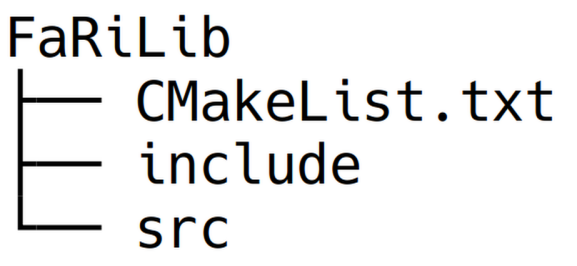
\includegraphics[width=0.8\linewidth]{assets/FaRiLibStructure.png}
            \label{fig:farilib_structure}
        \end{minipage}%
        \begin{minipage}{0.48\textwidth}
            \raggedright
            \begin{itemize}
                \item \textbf{CMakeLists.txt}: The CMake configuration file for the 
                library.
                \item \textbf{src/}: The source files of the library.
                \item \textbf{include/}: The header files of the library.
            \end{itemize}
        \end{minipage}
        \subsubsection{CMakeLists.txt}
        For the inclusion to work properly, a \texttt{CMakeLists.txt} file is
        necessary. It should contain the following lines: 
    \begin{lstlisting}[style=cppCode]
    project(FaRiLib)

    include_directories(include)

    set(SOURCE_FILES
            src/*
    )
    \end{lstlisting}
        In combination with the configuration done in section \ref{sec:farilib_include},
        this enables an include as simple as \texttt{\#include <FaRiLib.h>} in all
        node projects.

    \subsection{ESP NOW} \label{sec:farilib_espnow}
    The library provides a wrapper around the necessary ESP-NOW functionality.
    Functionally it is split into two header files, \texttt{espnowMaster.h} and 
    \texttt{espnowSlave.h}. The master node is the bridge node, while the slave
    nodes are the nodes that send data to the bridge node. Their exact implementation
    can be seen in section \ref{sec:node_implemtenation}.
        \subsubsection{ESP-NOW Objects}
        The aforementioned header files contain the \texttt{EspNowMaster} and the
        \texttt{EspNowSlave} classes. They both inherit from the abstract 
        \texttt{EspNow} class, which contains common functionality of both.
        \begin{figure}[H]
            \centering
            
\includegraphics[width=0.7\textwidth]{ThinkCorrectly.jpg}
            \caption{ESP-NOW Object Inheritance}
        \end{figure}

        \subsubsection{Device Discovery}
        The ESP-NOW discovery process is a crucial part of the system. It allows the
        bridge node to discover new nodes and allows the slave nodes to find the bridge
        node. The process is as follows:
        \begin{figure}
            \centering
            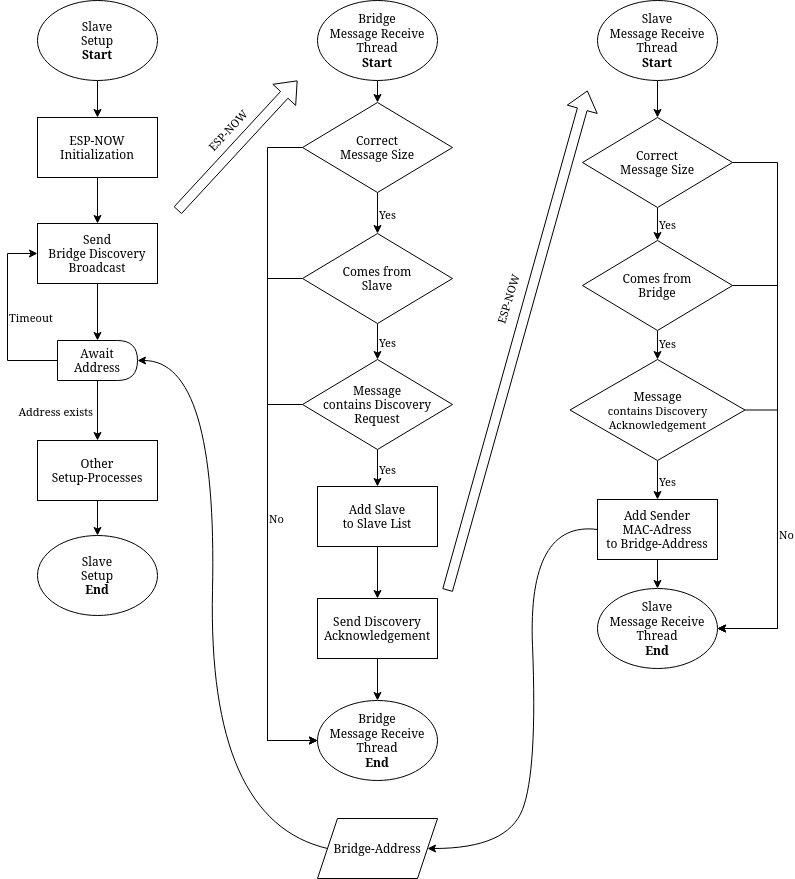
\includegraphics[width=\textwidth]{topics/flowcharts/ESP-NOW-Discovery.drawio.png}
            \caption{ESP-NOW Discovery Process}
            \label{fig:espnow_discovery}
            %THIS SHOULD BE REPLACED WITH A REAL DIAGRAM
        \end{figure}

    \subsection{HTTP} \label{sec:farilib_http}